\documentclass[12pt, svgnames]{book}

\usepackage{customPreamble}
\usepackage{customLanguages}

\centering

\title{\myfont Making a kernel}
\author{}
\date{}
\begin{document}
\pagenumbering{gobble}

\newcommand{\background}[1]{\tikz[remember picture,overlay] \node[opacity=1,inner sep=0pt] at (current page.center){\includegraphics[width=\paperwidth,height=\paperheight]{#1}};
	\clearpage}

\background{Cover.png}

\newpage

\maketitle

\newpage


\mainmatter
\pagenumbering{roman}
\tableofcontents

\newpage
\pagenumbering{gobble}
\pagenumbering{arabic}

\part{The tools}

\chapter*{Introduction and Setup}
\addcontentsline{toc}{chapter}{Introduction}

\section{Introduction}
This text is intended as both a log for the PiOS project and as a reference guide for anyone trying a similar project in the future. All text here is pertinent to the Raspberry Pi model 3 B, as this is the model we are using, past and different models may have different architectures, and as such, certain sections fo this guide may be useless for those working on those machines. This is not a documentation manual, for the PiOS documentation, please refer to the PiOS documentation manual.

\section{Hardware and Physical tools}
To start creating a kernel for the Raspberry Pi, the following is needed:

\begin{itemize}
	\item Raspberry Pi board (model 3 B is used in this document)
	\item Micro SD card 
	\item Micro USB adapter and cable to power the PI (5V @ 2A recommended)
	\item An independent machine with an operating system to compile the source code (aka PC) 
	\item A micro SD to USB adapter or any other method to store the compiled binaries into the micro SD card
\end{itemize}

The following is optional:

\begin{itemize}
	\item Raspberry Pi case
	\item JTAG system for debugging
	\item A monitor compatible with the Pi's video core
\end{itemize}

\section{Software}
\label{sec:Software}
The following software is needed to create the kernel:

\begin{itemize}
	\item Cross compiler to generate the binaries. Options include the \href{https://launchpad.net/\notengl{gcc}-arm-embedded}{GNU ARM Embedded Toolchain} (used in this document)
	\\
	\textcolor{red}{WARNING}: old \notengl{gcc} versions can generate problems with function attributes, it's recommended to use the latest \notengl{gcc} version.
	\item Raspberry Pi firmware binaries. In order for the boot process to be executed correctly it is needed to have the \href{https://github.com/raspberrypi/firmware/blob/master/boot/bootcode.bin}{bootcode.bin} and \href{https://github.com/raspberrypi/firmware/blob/master/boot/start.elf}{start.elf} binaries inside of the micro SD card.
	\item A text editor or IDE (no help will be provided as to how to setup an IDE)
\end{itemize}

It is also recommended that the reader has enough experience with \notengl{C} and ARM assembly, as it is assumed that the reader understands the syntax of these languages. An understanding of linker scripts is also helpful.

\section{Compilation}
\label{sec:compilation}
The following are the bare minimum commands needed to build a working kernel image. 
\\~\\
To compile \notengl{C} files:

\lstset{language=GCC}
\begin{lstlisting}[style = bash, xleftmargin=0\textwidth]
	arm-none-eabi-\notengl{gcc} -<opt> -<arch> <src> -o -c <o_file>
\end{lstlisting}

Where \compl{$<$opt$>$} refers to the level of optimization, \compl{$<$arch$>$} refers to the target architecture, \compl{$<$src$>$} is the source file(s) and \compl{$<$o\_file$>$} is the generated object file. The -c argument tells the compiler to generate the .o file without linking, this argument is VERY important, and things won't work without it.
\\~\\
Example:
\begin{lstlisting}[style = bash, xleftmargin=0\textwidth]
	arm-none-eabi-\notengl{gcc} -O0 -march=armv8-a source/MainFiles/PiTest.c -nostartfiles -c -o objects/MainFiles/PiTest.o
\end{lstlisting}

To compile ARM assembly files:
\begin{lstlisting}[style = bash, xleftmargin=0\textwidth]
	arm-none-eabi-as -<arch> <src> -c -o <o_file>
\end{lstlisting}

The flags here are the same as above, except that \compl{$<$src$>$} should be an ARM assembly file instead of a \notengl{C} file.
\\~\\
Example:
\begin{lstlisting}[style = bash, xleftmargin=0\textwidth]
	arm-none-eabi-as -march=armv8-a source/boot/boot.s -c -o objects/boot/boot.o
\end{lstlisting}

To link all object files:
\begin{lstlisting}[style = bash, xleftmargin=0\textwidth]
	arm-none-eabi-ld <o_file(s)> -o <elf> -T <linker(s)>
\end{lstlisting}

Where \compl{$<$o\_files$>$} refers to all object binaries that will makeup the final kernel image, \compl{$<$elf$>$} refers to the output .elf file and \compl{$<$linker(s)$>$} refers to all linker scripts (normally just 1), needed to link the objects.
\\~\\
Example:
\begin{lstlisting}[style = bash, xleftmargin=0\textwidth]
	arm-none-eabi-ld ./objects/MainFiles/PiTest.o ./objects/boot/boot.o  -o build/kernel.elf -T ./source/kernel.ld
\end{lstlisting}

To extract the raw image binary:
\begin{lstlisting}[style = bash, xleftmargin=0\textwidth]
	arm-none-eabi-objcopy <elf> -O binary <image>
\end{lstlisting}

Where \compl{$<$elf$>$} is the .elf file created on the above step and $<$image$>$ is the final kernel image binary. 
\\~\\
Example:
\begin{lstlisting}[style = bash, xleftmargin=0\textwidth]
	arm-none-eabi-objcopy build/kernel.elf -O binary kernel.img
\end{lstlisting}

To \hypertarget{dasm}{disassemble} the final .img binary for debugging:
\begin{lstlisting}[style = bash, xleftmargin=0\textwidth]
	arm-none-eabi-objdump -D <elf>
\end{lstlisting}

Although not necessary for compilation, it is recommended to execute and store the output of this command in a file, as it is very helpful for debugging and verifying the correctness of the final binary (.img).
\\~\\
Example:
\begin{lstlisting}[style = bash, xleftmargin=0\textwidth]
	arm-none-eabi-objdump -D build/kernel.elf > logs/kernel.list
\end{lstlisting}

For this project we also made use of \notengl{\notengl{C}++}, mainly to have the benefit of function overloading. However \notengl{g++}, the GNU \notengl{\notengl{C}++} compiler, which is used in this document, enables exceptions by default, which may cause some odd errors about certain functions not being found. In order to prevent this error from happening an additional argument must be given to the \notengl{g++} compiler to disable exceptions. The additional argument is:
\begin{lstlisting}[style = bash, xleftmargin=0\textwidth]
	-fno-exceptions
\end{lstlisting}

We will go into more detail in a \hyperref[sec:Programming Languages]{future section}.
\\~\\
For more information refer to the \href{https://\notengl{gcc}.gnu.org/onlinedocs/}{official GNU documentation} for your current version (or to the documentation of your toolchain).

\section{First Program}
\label{sec:first program}

After all prerequisites are met, it is necessary to verify that things work properly. This section simply provides a minimal example to test that all requirements were installed correctly. A more in depth explanation is provided on the \hyperref[sec:mailbox]{Mailbox} section.
\\~\\
To test whether everything is working fine, we just want to turn on the Pi's A\notengl{C}T LED on, however on the Pi 3, the led is not connected to the GPIO lines, so we have to communicate with the video core through the mailbox to turn it on. To be extra-sure everything is fine, we want it to blink. The following \notengl{C} code is used to send the appropriate message to the mailbox to turn the LED on.

\lstset{language=C}
\begin{lstlisting}[style=C]
	#include <stdint.h>
	
	#define REGISTERS_BASE 0x3F000000
	#define MAIL_BASE 0xB880  // Base address for the mailbox registers
	// This bit is set in the status register if there is no space to write into the mailbox
	#define MAIL_FULL 0x80000000
	// This bit is set in the status register if there is nothing to read from the mailbox
	#define MAIL_EMPTY 0x40000000
	
	struct Message
	{
		uint32_t messageSize;
		uint32_t requestCode;
		uint32_t tagID;
		uint32_t bufferSize;
		uint32_t requestSize;
		uint32_t pinNum;
		uint32_t on_off_switch;
		uint32_t end;
	};
	
	volatile struct Message m =
	{
		.messageSize = sizeof(struct Message),
		.requestCode =0,
		.tagID = 0x00038041,
		.bufferSize = 8,
		.requestSize =0,
		.pinNum = 130,
		.on_off_switch = 1,
		.end = 0,
	};
	
	/** Main function - we'll never return from here */
	int kernel_main(void)
	{
		uint32_t mailbox = MAIL_BASE + REGISTERS_BASE + 0x18;
		volatile uint32_t status;
		
		while(1)
		{
			do
				status = *(volatile uint32_t *)(mailbox);
			while((status & 0x80000000));
			
			*(volatile uint32_t *)(MAIL_BASE + REGISTERS_BASE + 0x20) = 
				((uint32_t)(&m) & 0xfffffff0) | (uint32_t)(8);
			
			int i=0;
			
			while(i<0xF0000)
				i++;
			
			if(m.on_off_switch == 0)
				m.on_off_switch = 1;
			
			else
				m.on_off_switch = 0;
			
			m.requestCode = 0;
			m.requestSize = 0;
			m.pinNum = 130;
			m.end = 0;
			
			do
				status = *(volatile uint32_t *)(mailbox);
			while((status & 0x40000000));
			
			uint32_t temp;
			
			do
				temp = *(uint32_t *)(MAIL_BASE + REGISTERS_BASE);
				temp = temp & 0xF;
			while(temp != 8);
		}
	}
\end{lstlisting}


As big as this seems for a ``hello world!" example, it is the smallest \notengl{C} code we could come up with that light the LED. And we are not even done yet. This code is using memory, and if one where to \hyperlink{dasm}{disassemble} the binaries, one could see that the sp register (stack pointer). Is used, as such we need to initialize it properly.

The following assembly initializes the stack pointer and branches to our main loop:
\lstset{language=ASM}
\begin{lstlisting}[style = ASM]
	.section .init
	.global _start
	
	_start:
		ldr sp, =8000
		b kernel_main
\end{lstlisting}

However we still are not done. The Raspberry Pi always begins execution at address \compl{0x8000}, so whatever instruction is at that address will be the first to run. We need to ensure this instruction is also the first instruction in the above code. For this we use the following linker file:

\lstset{language=Linker}
\begin{lstlisting}[style = C]
	SECTIONS 
	{
		.init 0x8000 : 
		{
		*(.init)
		}
		
		.text : 
		{
		*(.text)
		}
		
		.data ALIGN(0x20) : 
		{
		*(.data)
		}
	}
	
\end{lstlisting}

\textcolor{red}{WARNING:} Depending on the compiler, sections of the code could be optimized out, be wary of compiler optimization options.
\\~\\
If the reader doesn't fully understand what the \notengl{C} code is doing, it will be further explained in the following sections. However the functioning of linker scripts, or assembly language will not be explained.

\chapter{Understanding Compilation}

\section{Programming Languages}
\label{sec:Programming Languages}
Here we will discuss some important details of the different languages we will use in order to understand certain design choices we will later make.

\subsection{ARM}
Although the least used of the 3 languages, ARM assembly is the most important of the 3 languages used, since all of our source code will eventually become arm assembly code before being turned into machine code (a compiler, such as \notengl{gcc}, first turns the source code into assembly code, and it then calls an assembler to translate this assembly code into binary code). 
\\~\\
Specifically we care about the following things:
\\~\\
First there are hardware specific things that are not available at the \notengl{C} level and so we must use assembly to interact with them. Some examples of things that are not exposed to \notengl{C} are registers, special instructions like the ``change program state" \compl{cps} instruction, special registers like the stack pointer, link register, current program status register... and others.
\\~\\ 
Next we need to be aware that at the end of the day an assembly instruction in arm is nothing but a bit string, a sequence of 1's and 0's. As such there is no difference between an instruction and data as far as the CPU is concerned. For this we must be very careful to ensure that the program counter never holds a value that does not correspond to an instruction. 
\\
For example the value \compl{0x00000000}corresponds to the arm instruction\compl{andeq   r0, r0, r0} and the value \compl{0xe2833001} corresponds to the instruction \compl{add r3, r3, \#1}. 
\\
In addition to this, some values have no CPU instruction associated with them, they are undefined instructions and they will trigger an exception if loaded into the program counter.
\\
The program counter always loads the instruction at the next \compl{word} (i.e pc+4) so to prevent unexpected values from being loaded into the program counter we purposely add infinite loops at critical sections of the code. 

\subsection{\notengl{C}}

The first of the 2 high level languages that we use. There just a few things that we need to understand about the use of \notengl{C} in the project. 
\\~\\
First, \notengl{C} is very close to assembly. In fact, someone with enough experience could probably predict how a given \notengl{C} function will be compiled. This is important because we need to understand how \notengl{C} will be compiled into assembly to prevent errors and maximize our use of \notengl{C}. A common example is the fact that one can use pointers and structure definitions to abstract a given memory mapped peripheral such as the system timer. This is mostly self evident in the syntax so we will explain it further on the relevant sections.
\\~\\
Second we must be aware that all of our code lives in ram memory. As such the only thing differentiating a structure from a function is the code itself. A struct should never be used as a function, although it is perfectly possible to trick the \notengl{C} compiler to do it. So, as stated before, it is important to be aware that this high level abstractions, although convenient, don't exist once we are actually running our code. As an example in this \hyperlink{fig_example}{comparison} A function and an array get compiled identically to the same binary executable. 

\hypertarget{fig_example}{}

\begin{minipage}{0.5\textwidth}
	\lstset{framesep=53pt}
	\begin{lstlisting}[style=c-small, title= Function]
		void example()
		{
			int i = 0;
		
			i = 500;
		}
	\end{lstlisting}
\end{minipage}
\begin{minipage}{0.5\textwidth}
	\begin{lstlisting}[style=c-small, title= Array]
	unsigned int example[] =
	{
		0xe52db004,
		0xe28db000,
		0xe24dd00c,
		0xe3a03000,
		0xe50b3008,
		0xe3a03f7d,
		0xe50b3008,
		0xe1a00000,                     
		0xe28bd000,
		0xe49db004,   
		0xe12fff1e,
	};
	\end{lstlisting}
\end{minipage}
\begin{minipage}{0.5\textwidth}
	\begin{lstlisting}[style=disassembly,]
	00000000 <example>:
	0:    e52db004        push    {fp}
	4:    e28db000        add     fp, sp, #0
	8:    e24dd00c        sub     sp, sp, #12
	c:    e3a03000        mov     r3, #0
	10:   e50b3008        str     r3, [fp, #-8]
	14:   e3a03f7d        mov     r3, #500 
	18:   e50b3008        str     r3, [fp, #-8]
	1c:   e1a00000        nop                     
	20:   e28bd000        add     sp, fp, #0
	24:   e49db004        pop     {fp}   
	28:   e12fff1e        bx      lr
	\end{lstlisting}
\end{minipage}
\begin{minipage}{0.5\textwidth}
	\begin{lstlisting}[style=disassembly,]
	00000000 <example>:
	0:   e52db004        push    {fp}            
	4:   e28db000        add     fp, sp, #0
	8:   e24dd00c        sub     sp, sp, #12
	c:   e3a03000        mov     r3, #0
	10:   e50b3008        str     r3, [fp, #-8]
	14:   e3a03f7d        mov     r3, #500       
	18:   e50b3008        str     r3, [fp, #-8]
	1c:   e1a00000        nop                     
	20:   e28bd000        add     sp, fp, #0
	24:   e49db004        pop     {fp}            
	28:   e12fff1e        bx      lr
	\end{lstlisting}
\end{minipage}

\subsection{\notengl{C++}}
This is the final language that is used in this project. Although it is almost identical to \notengl{C} there are a few differences that need to be addressed to prevent errors due to incompatibility or missing libraries.
\\~\\
First of all, unlike \notengl{gcc}, \notengl{g++} enables exception handling by default. The most important aspect for us of this exceptions is the fact that the compiler assume s the existence of libraries and functions to handle an exception. It is possible that the code compiles just fine, but it's also natural that at some point during the compilation problem one sees at least one of the following errors:

\begin{lstlisting}[style=bash]
	undefined reference to `__aeabi_unwind_cpp_pr0'
\end{lstlisting}

\begin{lstlisting}[style=bash]
	undefined reference to `__aeabi_unwind_cpp_pr1'
\end{lstlisting}

Stack unwinding is used by exceptions, debuggers (e.g GDB) and by any program trying to display the call chain. In ARM this is done with the use of the sections \compl{.ARM.exidx} and \compl{.ARM.extab}. Although understanding this process is certainly important for the OS development it is not relevant to this section, but if one wishes to learn more there are external \href{https://wiki.linaro.org/KenWerner/Sandbox/libunwind?action=AttachFile&do=get&target=libunwind-LDS.pdf}{resources}.
\\~\\
Using compilation options such as\compl{-nostdlib}, \compl{-nostartfiles} and/or \compl{-nodefaultlibs} won't get rid of the error. However we cna prevent the error from happening very easily by including the option:

\begin{lstlisting}[]
	-fno-exceptions
\end{lstlisting}

Into our \notengl{g++} command line parameters, as previously discussed. 
\\~\\
The other important aspect of \notengl{C++} is name mangling. Unlike \notengl{C}, \notengl{C++} has object orientation and function overloading and overwriting. In \notengl{C} only one function definition with a given label may exist (such as printf()), but \notengl{C++} allows us to define multiple functions with the same name as long as their signatures are different. In example one may define:

\begin{lstlisting}[style=C]
	void function(int num)
	{
		/* code */
	}
	void function(char character)
	{
		/* code */
	}
\end{lstlisting}

In the same \notengl{C++} source code with no problems. This is all due to name mangling. In reality 2 functions cannot share the same name, but \notengl{C++} goes around this restriction by changing the names of functions and adding extra information such as the number and type of parameters to a functions name, thus guaranteeing that functions with the same name but different signature will be considered as different labels by the assembler.
\\~\\
Take for example the following function, which is defined in a \notengl{C} file (i.e .c extension). We can see how differently the \notengl{gcc} and \notengl{g++} have compiled the funtion label:

\centering
\begin{minipage}{0.45\textwidth}
	\begin{lstlisting}[style=c, title= Source]
		void function()
		{
		
		}
	\end{lstlisting}
\end{minipage}

\begin{minipage}{0.45\textwidth}
	\begin{lstlisting}[style=bash, title= \notengl{gcc}]
	00000000 <function>:
	0:   e52db004        push    {fp}           
	4:   e28db000        add     fp, sp, #0
	8:   e1a00000        nop                     
	c:   e28bd000        add     sp, fp, #0
	10:   e49db004        pop     {fp}            
	14:   e12fff1e        bx      lr
	\end{lstlisting}
\end{minipage}
\begin{minipage}{0.45\textwidth}
	\begin{lstlisting}[style=bash, title= \notengl{g++}]
	00000000 <_Z8functionv>:
	0:   e52db004        push    {fp}            
	4:   e28db000        add     fp, sp, #0
	8:   e1a00000        nop                    
	c:   e28bd000        add     sp, fp, #0
	10:   e49db004        pop     {fp}           
	14:   e12fff1e        bx      lr
	\end{lstlisting}
\end{minipage}

\section{Language integration}

\flushleft
The reason why we care about this things is because we are integrating all 3 languages and we are using \notengl{C} and Assembly, which do not name mangle. This means that these languages would be unaware of the existence of \notengl{C++} functions, mainly because if one writes:

\begin{lstlisting}[style=C]
	void main(void)
	{
		cppFunc();
	}
\end{lstlisting}

In a \notengl{C} program, where \compl{cppFunc()} is a \notengl{C++} function, the \notengl{C} program expects exactly the label \compl{cppFunc}, but due to name mangling the function will have a different name as we have already seen. There are 2 things we will do to make the 3 languages work together.
\\~\\
First, although it is possible to use a combination of \notengl{gcc} and \notengl{g++} to compile source code, for simplicity we decided to use \notengl{g++} as a compiler for both \notengl{C} and \notengl{C++} source files, this fully integrates \notengl{C} and \notengl{C++}, since the \notengl{g++} compiler understands name mangling, and as such, even if a \notengl{C++} function is called in a \notengl{C} file, it will compile properly, which is easier than working with 2 compilers at a time.
\\~\\
Secondly, the assembly code however doesn't need to be compiled, only assembled. This is done by invoking the arm assembler, so the problem of name mangling appears once more. An instruction such as \compl{b func} won't be assembled correctly if \compl{func} is defined in a file compiled by the \notengl{g++} compiler, as this label will be changed by the compiler. Fortunately there is a way around this. the use of the \compl{extern ``C"} key\compl{word} allows us to tell the \notengl{g++} compiler to avoid name mangling a specific function or set of functions. There are 2 ways of using it:
\\~\\
\newbox\longbox
\newbox\shortbox
\setbox\longbox=\vbox{
	\hsize=.48\linewidth
	\begin{lstlisting}[style=C, linewidth=\hsize]
	extern "C" {
	void function()
	{
		/* code */
	}
	}
	\end{lstlisting}
	\hrule height0pt
}
\setbox\shortbox=\vbox to\ht\longbox{
	\hsize=.48\linewidth
	\begin{lstlisting}[style=C, linewidth=\hsize]
	extern "C" void function()
	{
		/* code */
	}
	\end{lstlisting}
	\vfill
}
\noindent
\hbox to\linewidth{%
	\colorbox{deepblue}{\box\shortbox}%
	\hfil
	\colorbox{deepblue}{\box\longbox}%
}
\\~\\
For the right option, any function declared inside of the curly brackets will not be named mangled, so it is very suitable to use this in header files. No matter which of the 2 we use however, the function will be labeled as is, so in both cases the generated assembly code would have this function defined as \compl{function}. There is an alternative which is to see how functions get mangled by \notengl{g++} and then use those labels in the assembly code, but this is tedious and has the issue that if we change a function's signature, the assembled label will change as well and we would have to change the assembly code as well, which is inefficient. 

\section{Compilation}

Although briefly, we need to discuss compilation especially because we will be making our own compilation script.

The compilation process is fairly straightforward, and can be summarized as follows:
\begin{enumerate}
	\item The macroprocessor replaces all macros:
	At this point all \compl{\#define}, \compl{\#includes} and other macros get replaced. The only thing we are worried about here is to make sure the proper include guards are defined in all header files to prevent redefinitions of symbols.
	
	\item The compiler generates assembly code:
	At this stage the compiler will take all macro replaced temporal files and will generate assembly code for the target architecture.
	
	\item The compiler assembles the assembly code:
	At this stage the compiler invokes the assembler, which takes the temporal assembly files and generates a permanent, final binary file (usually object files with the \notengl{.o} extension).
	
	\item The linker links everything together:
	At the final stage, the linker is invoked and takes all object files and combines them together to create a final binary executable.
\end{enumerate}

The reason why we must understand the compilation process properly, is because we will not be using the default linking script that \notengl{g++} uses, but rather we will make our own. This is because we need to create certain labels, define some custom, special sections, and discard unused sections that may be created by default but that we are not using to reduce the final size of our executable. This will become apparent in future sections.

The final linking script looks like:
\\~\\
\hypertarget{linker script}{}
\begin{lstlisting}[style=C, language=Linker, title=Co-Edited with \href{https://www.raspberrypi.org/forums/memberlist.php?mode=viewprofile&u=213434}{Leon de Boer}, captionpos=b]
	SECTIONS 
	{
		.init 0x8000 : 
		{
			KEEP(*(.init))
		}
		
		.text : 
		{
			. = ALIGN(4);
			__text_start__ = .;              
			*(.text .text.* .gnu.linkonce.t.*)
			. = ALIGN(4);
			__text_end__ = .;               
		}
		
		.data : 
		{
			. = ALIGN(4);
			__data_start__ = .;           
			*(.data .data.* .gnu.linkonce.d.*)
			. = ALIGN(4);
			__data_end__ = .;            
		}
		
		.bss :
		{
			. = ALIGN(4);
			__bss_start__ = .;
			KEEP(*(.bss))
			. = ALIGN(4);
			__bss_end__ = .;
		}
		
		/* Made by LDB */
		.stack :
		{
			. = ALIGN(8);  
			__stack_start__ = .;
			. = . + 512;    /* fiq stack size */
			__fiq_stack = .;
			. = . + 16384;   /* usr & sys stack size (common) */
			__usrsys_stack = .;
			. = . + 16384;  /* svc stack size (start-up) */
			__svc_stack = .;
			. = . + 4096;   /* irq stack size */
			__irq_stack = .;
			. = . + 512;    /* mon stack size */
			__mon_stack = .;
			. = . + 512;    /* hyp stack size */
			__hyp_stack = .;
			. = . + 512;    /* und stack size */
			__und_stack = .;
			. = ALIGN(8);
			__stack_end__ = .;      
		}
		/* end of LDB contribution */
		
		.Heap :
		{
			. = ALIGN(4);
			Kernel_End = .;     /* Label to mark end of kernel code*/; 
		}
	}
\end{lstlisting}

	Which simply defines an \compl{init} section for \hyperref[sec:Setting up the hardware]{second stage booting} the standard \compl{data}, \compl{text} and \compl{bss} sections, allocates some RAM space for the different stacks of the exception modes since each uses a different stack pointer and then finally creates a label to know where the end of the kernel space is and where the start of the heap space begins.
	 
\part{Making the kernel}

\chapter{Booting}

\section{Raspberry Pi firmware}

As mentioned in a previous  \hyperref[sec:Software]{previous section}, the first steps of booting are done with the help of some firmware. Basically the Video Core is responsible to do the first stage booting, which will initialize one of the cores and load the kernel binary into the core to begin execution.
\\~\\
We could customize this process with he help of a configuration file called \notengl{config.txt} which would do help configure the hardware; for example we could select a custom file as the selected kernel instead of using the default names. However we will leave it aside for now. More information about the \notengl{config.txt} file it can be found in the \href{https://www.raspberrypi.org/documentation/configuration/config-txt/}{offical site of the Pi organization}.
\\~\\
What we care about mostly, is that the name of our kernel binary affects how it is loaded into RAM. If we don't use the configuration file then, for the Raspberry Pi 3, the firmware will look for a list of file names in a priority order to load into RAM, the order, from first to last is:
\notengl{kernel8.img} (boots into 64 bit mode, all other boot into 32 bit mode), \notengl{kernel8-32.img}, \notengl{kernel7.img}, \notengl{kernel.img}. This is simply so that one may load all 3 different kernel versions into the same SD card and all models of the pi would find their corresponding kernel image and load that one, for simplicity purposes however and since we are only working on a pi 3, we named our kernel image \notengl{kernel.img}.
\\
No matter the kernel version, without a configuration file they all start executing whatever instruction is loaded at RAM address \compl{0x8000}, which is why we made sure in our \hyperlink{linker script}{linker script} to load the \compl{init} section at that address.

\section{Setting up the hardware}
\label{sec:Setting up the hardware}

At this point the firmware has already finished loading the kernel image executable into ram and has initialized the program counter to the appropriate value (\compl{0x8000} in our case). However the Video Core has done the minimum work to set up the hardware, only one core has been properly initialized, the floating point unit has not been set up... So we need to make sure to initialize everything properly ourselves.

\subsection{Installing the Interrupt Vector Table (IVT)}
\label{sec:IVT}
The first thing we want to do is initialize the Interrupt Vector Table. In the Raspberry Pi 3, when an exception is triggered, a specific address's content gets loaded into the program counter, although it is actually possible to specify the location of the IVT, by default this is it's configuration:
\begin{center}
\arrayrulecolor{deepblue}
{\rowcolors{1}{lightblue!100}{pastelblue!100}
\begin{tabular}{ |c|c|c| }
	\hline
	RAM address & Exception Type 		& Execution Mode	\\
	\hline
	0x00		& Reset					& Supervisor		\\
	0x04		& Undefined Instruction	& Undefined			\\
	0x08		& Software Interrupt	& Supervisor		\\
	0x0C		& Prefetch Abort 		& Abort				\\
	0x10		& Data abort 			& Abort				\\
	0x14		& Reserved				& (Reserved for future expansion)\\
	0x18		& Interrupt (IRQ)		& IRQ					\\
	0x1C		& Fast Interrupt (FIQ) 	& FIQ					\\
	\hline
\end{tabular}
}
\end{center}

Due to the fact that there is no space in between each table entry, the table consists of branch instructions that jump to a subroutine in a different section of memory, and this subroutine handles the exception and returns if and when appropriate.
\\~\\
We will talk more about this in the \hyperref[sec:Interrupts]{Interrupts section}, for the moment all that we want to do is to  make sure the correct values are installed in these first 8 \compl{word}s in RAM.

The assembler considers labels to be relative to the PC position, thus if we simply try to load something like \compl{ldr pc, =exception\_handler} into the vector table, there will be a problem as this instruction will look like \compl{ldr pc, [pc, \#offset]}. The way around it is to create a set of labels containing the actual RAM positions of the exception handling routines immediately after the branch instructions and load their values into low memory as well to keep the same relative offset. In other \compl{word}s, in our data section we define \hyperlink{IVT}{this structure}.
\\
And then we simply load both the instructions and the subroutine addresses together into low memory as follows: 

\begin{lstlisting}[language=ASM, title={Code taken from the \href{http://www.valvers.com/open-software/raspberry-pi/step04-bare-metal-programming-in-c-pt4/}{Valvers Ttorial}},captionpos=b]
	_start:
	_reset_:
		ldr     r0, =_v_table
		mov     r1, #0x0000
		ldmia   r0!,{r2, r3, r4, r5, r6, r7, r8, r9}
		stmia   r1!,{r2, r3, r4, r5, r6, r7, r8, r9}
		ldmia   r0!,{r2, r3, r4, r5, r6, r7, r8, r9}
		stmia   r1!,{r2, r3, r4, r5, r6, r7, r8, r9}
\end{lstlisting}

\newpage

\hypertarget{IVT}{}
\begin{lstlisting}[language=ASM, title=IVT Structure, title={Code taken from the \href{http://www.valvers.com/open-software/raspberry-pi/step04-bare-metal-programming-in-c-pt4/}{Valvers Ttorial}},captionpos=b]
	_v_table:
		ldr     pc, _reset_h
		ldr     pc, _undefined_instruction_vector_h
		ldr     pc, _software_interrupt_vector_h
		ldr     pc, _prefetch_abort_vector_h
		ldr     pc, _data_abort_vector_h
		ldr     pc, _unused_handler_h
		ldr     pc, _interrupt_vector_h
		ldr     pc, _fast_interrupt_vector_h
		
	_reset_h:                            .\compl{word}   _reset_
	_undefined_instruction_vector_h:     .\compl{word}   undefined_instruction_vector
	_software_interrupt_vector_h:        .\compl{word}   software_interrupt_vector
	_prefetch_abort_vector_h:            .\compl{word}   prefetch_abort_vector
	_data_abort_vector_h:                .\compl{word}   _reset_
	_unused_handler_h:                   .\compl{word}   _reset_
	_interrupt_vector_h:                 .\compl{word}   interrupt_vector
	_fast_interrupt_vector_h:            .\compl{word}   fast_interrupt_vector
\end{lstlisting}

Once this is done, the next step is to setup the execution mode. The Pi boots into Hypervisor mode, however although this mode has the highest privilege level, it cannot do certain things. Normally when we want to change modes we would use the \compl{CPS} (Change Program State) instruction, but this will trigger exception on the Pi 3 when trying to switch out of Hypervisor mode, the way to actually switch to Supervisor mode was generously provided provided by Leon de Boer as the following subroutine:

\begin{lstlisting}[language=ASM, title={Code provided by \href{https://www.raspberrypi.org/forums/memberlist.php?mode=viewprofile&u=213434}{Leon de Boer}},captionpos=b]
	RPi_CheckAndExitHypModeToSvcMode:
	mrs r0, cpsr               ;@ Fetch the cpsr register             
	and r1, r0, #0x1F          ;@ Mask off the arm mode bits in register                            
	cmp r1, #0x1A              ;@ check we are in HYP_MODE AKA register reads 1A                     
	beq .WeHaveHyperMode
	mov r0, #0;                ;@ return false
	bx lr                      ;@ Return we are not in hypermode
	.WeHaveHyperMode:
	bic r0, r0, #0x1F          ;@ Clear the mode bits                   
	orr r0, r0, #0xD3          ;@ We want SRV_MODE with IRQ/FIQ disabled         
	mov r1, #0                 ;@ Make sure CNTVOFF to 0 before exit HYP mode
	mcrr p15, #4, r1, r1, cr14 ;@ We do not want our clocks going fwd or bwd
	orr r0, r0, #0x100         ;@ Set data abort mask    
	msr spsr_cxsf, r0          ;@ Load our request into return status register
	mov r0, #1;                ;@ return true
	
	.long 0xE12EF30E                  ;@ "msr ELR_hyp, lr"
	.long 0xE160006E                  ;@ "eret"   
\end{lstlisting}

It can be summarized as, checking if the CPU is running in Hypervisor mode, if it is then we switch to supervisor mode. The exact details as to why this must be done in this specific way are not discussed here.

\subsection{Initializing the stacks}

Now that we are in Supervisor mode, we can properly set up the stacks of the different execution modes (On the Pi 3 this is not possible in Hypervisor mode). 
\\~\\
Each of the execution modes has a different stack pointer, so we need to ensure that each of these points to a reserved location in RAM, that is big enough to hold the stack for that execution mode. In other \compl{word}s things like exceptions, which should execute fast and then exit, don't need big stacks, but the supervisor mode however will need a relatively large stack, as it's where the kernel executes. Thanks to our \hyperlink{linker script}{linker script}, we have labels to sections of memory we know are good enough to store the different stacks, so all we need is to properly initialize the stack pointers to these labels, which is very straightforward:

\sethlcolor{lightblue}
\begin{lstlisting}[language=ASM,title={Code provided by \href{https://www.raspberrypi.org/forums/memberlist.php?mode=viewprofile&u=213434}{Leon de Boer}},captionpos=b]
	msr CPSR_c, #0xD1                  ;@ Switch to FIQ_MODE
	ldr sp, =__fiq_stack               ;@ Set the stack pointer for that mode to 0x7000
	msr CPSR_c, #0xD2                  ;@ Switch to IRQ_MODE
	ldr sp, =__irq_stack               ;@ Set the stack pointer for that mode to 0x6000
	msr CPSR_c, #0xD3                  ;@ Switch back to SRV_MODE
	ldr sp, =__svc_stack               ;@ Set the stack pointer for that mode to 0x5000
\end{lstlisting}

\sethlcolor{lightgrey}

\subsection{Initializing hardware}

Finally, there are some things in the hardware that are not initialized by the Video Core that we need to initialize ourselves. Most of theses are not mandatory, but they will make code execution much faster, so it is worth the trouble.

The things we want to do ar basically, initializing the Floating Point Unit so that we can use floating point numbers, enabling branch prediction to accelerate the flow of the program and enable the caches for faster memory access for commonly used variables.
\\
Here we would also initialize the other cores but we didn't reach that point.
\\~\\
This can all be done sequentially and each thing is relatively small, so we will simply provide the code snippets necessary for these processes.
\newpage
 \begin{itemize}
 	\item Initializing the FPU
 	\begin{lstlisting}[language=ASM,title={Code provided by \href{https://www.raspberrypi.org/forums/memberlist.php?mode=viewprofile&u=213434}{Leon de Boer}},captionpos=b]
	 	mrc p15, 0, r0, c1, c1, 2          ;@ Read NSACR into R0
	 	cmp r0, #0x00000C00                ;@ Access turned on or in AARCH32 
	 	                                   ;@ mode and can not touch register or EL3 fault
	 	beq .free_to_enable_fpu
	 	orr r0, r0, #0x3<<10               ;@ Set access to both secure and 
		                                   ;@ non secure modes
	 	mcr p15, 0, r0, c1, c1, 2          ;@ Write NSACR
 	
 	.free_to_enable_fpu:
	 	mrc p15, 0, r0, c1, c0, #2          ;@ R0 = Access Control Register
	 	orr r0, #(0x300000 + 0xC00000)      ;@ Enable Single & Double Precision
	 	mcr p15,0,r0,c1,c0, #2              ;@ Access Control Register = R0
	 	mov r0, #0x40000000                 ;@ R0 = Enable VFP
	 	vmsr fpexc, r0                      ;@ FPEXC = R0
 	\end{lstlisting}
 	
 	\item Enable the caches and Branch Prediction
 	\begin{lstlisting}[language=ASM,title={Code provided by \href{https://www.raspberrypi.org/forums/memberlist.php?mode=viewprofile&u=213434}{Leon de Boer}},captionpos=b]
	 	mrc p15,0,r0,c1,c0,0               ;@ R0 = System Control Register
 	
 	#define SCTLR_ENABLE_DATA_CACHE         0x4
 	#define SCTLR_ENABLE_BRANCH_PREDICTION   0x800
 	#define SCTLR_ENABLE_INSTRUCTION_CACHE  0x1000
 	
	 	// Enable caches and branch prediction
	 	orr r0, #SCTLR_ENABLE_BRANCH_PREDICTION
	 	orr r0, #SCTLR_ENABLE_DATA_CACHE
	 	orr r0, #SCTLR_ENABLE_INSTRUCTION_CACHE
 	
	 	mcr p15, 0, r0, c1, c0,0               ;@ System Control Register = R0
 	\end{lstlisting}
 \end{itemize}
 
 To see a final, working implementation of all of these features, you can refer to the \href{https://github.com/Makogan/PiOS/blob/master/source/boot/boot.S}{\notengl{Boot.s}} file in the \href{https://github.com/Makogan/PiOS/tree/master/source}{PiOS source code}.

\section{Software initialization, the \notengl{\_cstartup} routine}

In a fully implemented Operating System, any global variables that need to be initialized before they are used, and any library initialization code needs to be called before these libraries cna be used. In our modest project, there are only a couple of libraries, but they need to be initialized nonetheless. Also, the \compl{bss} section must be cleared (i.e we must write a 0 to all addresses in the section). All of this is done in the \compl{\_cstartup} function.
\\
Although very humble in it's current state, if the project is extended so that more functionality is added, this is where we would call any library initialization code, in order to ensure that everything is setup before any function in a library gets called. 
\\~\\
The very first thing we want to do is clear the \compl{bss} section. Thanks to our \hyperlink{linker script}{linker script}, we have a label to indicate exactly where this section begins and another label to indicate exactly where it ends, the script also ensures that all \compl{bss} sections of all files get contiguously put together in the final kernel image, so we know that, once we clear this section, all variables that need to be initialized to 0 will contain their correct values. Since the addresses form a continuous block of memory, we can easily do his with a loop:

\begin{lstlisting}[style = C]
	volatile uint32_t* current_address = &__bss_start__;
	uint32_t* end = &__bss_end__;
	
	while(current_address < end)
	{
		*current_address = 0;
		current_address++;
	}
\end{lstlisting}

The next step is to sequentially call any initialization code from all libraries, and then go to the main kernel loop. So the final code would look like:

\begin{lstlisting}[style = C]
	void _cstartup()
	{
		/* clear bss section */
		
		/* initialize all libraries */
		init_lib1();
		init_lib2();
		init_lib3();
		[...]
		
		kernel_main();
		
		while(1){}
	}
\end{lstlisting}

We add an infinite loop at the end as a precaution. The main kernel routine should never return, but if for any reason it did, this prevents the program counter from being loaded with random values (which could even damage the hardware).
\\~\\
The final implementation for the PiOS project can be seen in the \href{https://github.com/Makogan/PiOS/blob/master/source/boot/cstartup.c}{\notengl{cstartup.c}} file.

\chapter{Peripherals}

Now that we have initialized the hardware and our libraries we can start doing some I/O.

\section{Mailbox}
\label{sec:mailbox}

The most important peripheral is probably the Mailbox. Most communication with non default peripherals such as monitors and USB peripherals is done through this device. Although officially there are 2 mailboxes on the Pi 3, it is unclear what the purpose of the second mailbox is, so for the sake of this document, it can be assumed that whenever we talk about the mailbox we are referring to the first one. 

\subsection{Mailbox Property Interface}

Communicating with the mailbox is a complex task and may be confusing. First there are 10 channels defined for communication with this device:

\begin{center}
	\arrayrulecolor{darkred}
	{\rowcolors{1}{red!30}{red!20}
		\begin{tabular}{ |c|c| }
			\hline
			Channel 	&	Name \\
			\hline
			0& Power management\\
			1& Framebuffer\\
			2& Virtual UART\\
			3& VCHIQ\\
			4& LEDs\\
			5& Buttons\\
			6& Touch screen\\
			7& Undefined\\
			8& Property tags (ARM to VC)\\
			9& Property tags (VC to ARM)\\
			\hline
		\end{tabular}
	}
\end{center}

But we will only focus on channel 8, since the other channels tend to behave strangely. We also must be aware of how the device is mapped to memory, which for all 3 models can be expressed as:

\begin{center}
	\arrayrulecolor{darkred}
	{\rowcolors{1}{red!30}{red!20}
		\begin{tabular}{ |c|c| }
			\hline
			Address 	&	Register \\
			\hline
			BASE + 0x00 & read\\
			BASE + 0x04 & unused\\
			BASE + 0x08 & unused\\
			BASE + 0x0C & unused\\
			BASE + 0x10 & Poll\\
			BASE + 0x14 & Sender\\
			BASE + 0x18 & Status\\
			BASE + 0x1c & Configuration\\
			BASE + 0x20 & Write\\
			\hline
		\end{tabular}
	}
\end{center}

For all 3 models the mailbox base address is \compl{0xB880} and the peripheral address for the Pi 3 is \compl{0x3F000000}, so the BASE variable in the above table should be \compl{0x3F00B880}.
\\~\\
Reading and writing to the mailbox are always done in the same fashion:

\begin{itemize}
	\item Reading
	\begin{enumerate}
		\item Read status register until the Mailbox isn't empty.
		\item Red the data from the read register
		\item Check the lower four bits to see if they match the desired channel, if not go to 1.
		\item Clear the lower 4 bits, the data is in the 28 most significant bits.
	\end{enumerate}
	\item Writing
	\begin{enumerate}
		\item Read status register until the Mailbox isn't full.
		\item Write the data along with the channel, which is stored in the 4 less significant bits.
	\end{enumerate}
\end{itemize}

Note that, because the channel is stored in the lowest 4 bits, the data must be 16 byte aligned to ensure the lower 4 bits are all 0. A more in depth explanation can be found on a \href{https://github.com/raspberrypi/firmware/wiki/Accessing-mailboxes}{Github Repository} but it should be taken with a grain of salt as there are mistakes on the documentation, and it is outdated for the Pi 3.

\newpage

\begin{lstlisting}[style=C, title = Reading]
	uint32_t read_from_mailbox(Channel channel)
	{
		uint32_t status;
		
		do
			status = *(volatile uint32_t *)(MAIL_BASE + IO_BASE + 0x18);
		while((status & MAIL_EMPTY));
		
		uint32_t response;
		
		do
			response = (*(uint32_t *)(MAIL_BASE + IO_BASE));
		while((response & 0xF) != channel);
		
		return response & ~0xF;
	}
\end{lstlisting}

\begin{lstlisting}[style=C, title = Writing]
	void write_to_mailbox(uint32_t message, Channel channel)
	{
		uint32_t status;
		
		do
			status = *(volatile uint32_t *)(MAIL_BASE + IO_BASE + 0x18);
			while((status & MAIL_FULL));
			
			*(volatile uint32_t *)(MAIL_BASE + IO_BASE + 0x20) = (((uint32_t)(message) & ~0xF) | (uint32_t)(channel));
	}
\end{lstlisting}

\subsection{Mailbox Messages}

When we wish to write to the mailbox, we must create a contiguous message in memory that specifies the information we are sending to the mailbox, and what we write to the Mailbox is the address of this message, combined with the channel, as seen before.

There is a general pattern for all messages as follows:
\begin{itemize}
	\item Message size in bytes.
	\item Request/Response code.
	\item Sequence of concatenated tags.
	\item 0x0 (End tag).
\end{itemize}

The request code is 0, and we should always write this value when sending a message, the 2 possible response codes are \compl{0x80000000} for a successful response and \compl{0x80000001} for an error.

The general pattern for a single tag is:

\begin{itemize}
	\item Tag identifier.
	\item Length of the value buffer in bytes.
	\item Length of the response buffer (overlaps value buffer) in bytes.
	\item Value/Response buffer.
\end{itemize}

For simplicity and convenience we can make all values are the size of a \compl{word}. So as to consider all of them 32 bit long numbers. The most general example for a mailbox message would be:

\begin{center}
	{\rowcolors{1}{grey!30}{grey!20}
		\begin{tabular}{c l l}
			u32:	&Size &\\
			u32:	&0x0	&\\	
			&	u32: &Tag 1\\
			&	u32: &Request size\\
			&	u32: &Response size\\
			& 	u32: &Start of Value/Response buffer\\
			&	\multicolumn{1}{c}{\vdots}	&\\
			&	u32:	& End of Value/Response buffer\\
			&	u32: &Tag 2\\
			&	u32: &Request size\\
			&	u32: &Response size\\
			& 	u32: &Start of Value/Response buffer\\
			&	\multicolumn{1}{c}{\vdots}	&\\
			&	u32:	& End of Value/Response buffer\\
			\multicolumn{1}{c}{\vdots} & &\\
			u32: & 0x0 &\\
			
		\end{tabular}
	}
\end{center}

A detailed explanation of most tags can be found on the official \href{https://github.com/raspberrypi/firmware/wiki/Mailbox-property-interface}{Github Page} But once again, there are mistakes so one should be weary.

The complete list of all tags defined on the pi 3 is given as an \hyperlink{Mailbox Tags}{appendix}.

A good way to test the Mailbox is to set the ACT LED , which can be done with the following example code:
\newpage
\begin{lstlisting}[style=C]
	uint32_t mailbox_message[8] __attribute__ ((aligned (16)));
	uint32_t index;
	
	void set_LED(int value)
	{
		// Set the default message values
		index = 1;
		mailbox_message[index++] =0, //request
		mailbox_message[index++] = (uint32_t) SET_GPIO_STATE, //tag
		mailbox_message[index++] = 8, //request size
		mailbox_message[index++] = 0, // response size
		mailbox_message[index++] = 130, //pin num
		mailbox_message[index++] = value, //state ON or OFF
		mailbox_message[index++] = 0, //end tag
		
		mailbox_message[0] = index*sizeof(uint32_t); //Total message size
		
		write_to_mailbox(((uint32_t) &mailbox_message | BUS_MASK), PTAG_ARM_TO_VC);
		read_from_mailbox(PTAG_ARM_TO_VC);
	}
\end{lstlisting}

\newpage
\subsection{Framebuffer}

The most important use of the Mailbox for us, is it's ability to communicate to an HDMI connected monitor. A framebuffer is a contiguous section of memory that the Video Core reads information from and writes this information to the monitor. In other \compl{word}s, it's a 1 dimensional array that is mapped to a 2 dimensional space, where each entry in the array corresponds to a pixel in the screen.
\\~\\
\centering
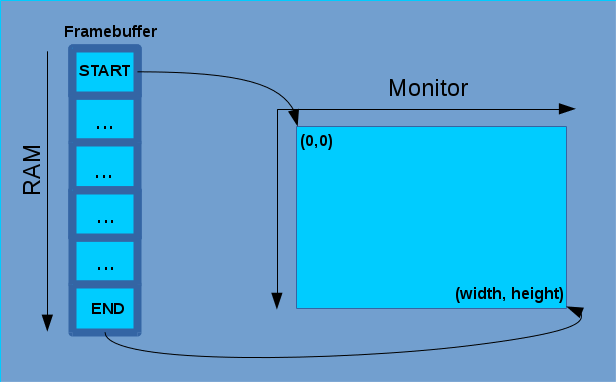
\includegraphics[scale=1]{FramebufferDiagram.png}

\flushleft
For things to work properly we must know beforehand the dimensions of the monitor we will be working with. Then we can set a virtual display whose dimensions are independent from the actual resolution of the monitor, for example we could make the virtual display 4 times smaller than the monitor, and as such each virtual pixel would correspond to 4 real pixels.
\\~\\
However, for simplicity, we will initialize the framebuffer such that the dimensions match the monitor's and we will also make it so that the color depth is 32 bits, such that each \compl{word} in the framebuffer corresponds to a pixel. There are 4 tags relevant to the framebuffer initialization process, set the physical dimensions, set the virtual dimensions, set the color depth and allocate the framebuffer in memory. This last one is important, as, unlike a desktop computer, the Raspberry Pi shares RAM with the Video Core, so we want to avoid  accidentally overwriting the data. Fortunately the Video Core returns not only the address of the framebuffer, but its size in bytes, so we can easily calculate it's boundaries.
\\~\\
For both the physical dimensions, virtual dimensions and color tags, the Video Core May not set the same values as the message depending on a variety of factors, the actual set values are returned at the same addresses as where they were sent (e.g the set physical width is returned on the same address as where the requested physical width was). The framebuffer tag also allows to specify the allignment of the allocated framebuffer on the same address as where the framebuffer pointer will be returned. 
\\~\\
A possible way to create this message is as follows.

\begin{lstlisting}[style =C]
	uint32_t mailbox_message[22] __attribute__ ((aligned (16)));
	uint32_t index;
	
	void set_init_display_message()
	{
		index = 1;
		mailbox_message[index++] = 0;//request code
		
		mailbox_message[index++] = (uint32_t) SET_PHYSICAL_WIDTH_HEIGHT; //tag
		mailbox_message[index++] = 8;	//request size
		mailbox_message[index++] = 8;	//response size
		mailbox_message[index++] = physical_width;	//horizontal resolution of the monitor
		mailbox_message[index++] = physical_height;	//vertical resolution of the monitor
		
		mailbox_message[index++] = (uint32_t) SET_VIRTUAL_WIDTH_HEIGHT;	//tag
		mailbox_message[index++] = 8;	//rquest size
		mailbox_message[index++] = 8;	// response size
		mailbox_message[index++] = virtual_width;	//horizontal resolution of virtual screen
		mailbox_message[index++] = virtual_height;	//vertical resolution of virtual screen
		
		mailbox_message[index++] = (uint32_t) SET_DEPTH;	//tag
		mailbox_message[index++] = 4;	//request size
		mailbox_message[index++] = 4;	//response size
		mailbox_message[index++] = color_depth;	//color depth of the frame buffer
		
		mailbox_message[index++] = (uint32_t) ALLOCATE;	//tag
		mailbox_message[index++] = 8;	//request size
		mailbox_message[index++] = 8;	//response size
		mailbox_message[index++] = 16;	//alignment fb ptr returned here
		mailbox_message[index++] = 0;	//fb size returned here
		
		mailbox_message[index++] = END;//end tag
		
		mailbox_message[0] = index*sizeof(uint32_t);	//size of message
	}
\end{lstlisting}

After this we simply write the message's address to the mailbox as previously explained and everything should be set. A fully working implementation for setting and using a framebuffer can be found on the \href{https://github.com/Makogan/PiOS/blob/master/source/Hardware/Graphics/mailbox.cpp}{\notengl{mailbox.cpp}} file in the PiOS source code.

\section{System timer}

The next peripheral we want to focus on is the system timer. There are actually multiple clocks on the Raspberry Pi located at different address, some are used by the ARM CPU, others by the Video Core. The one we are using is supposed to be very stable and it's what \href{http://embedded-xinu.readthedocs.io/en/latest/arm/rpi/}{Embedded Xinu} uses to keep track of time.
\\~\\
The system timer runs by default at 1.2 GHz, so for convenience and simplicity we can assume that 1 million cycles are 1 second (this is quite obviously wrong and would cause issues in a real time OS, but for our humble project it's good enough), the actual relation is that 1.2 million cycles are 1 second, so we are somewhat close.
\\~\\
On the Pi 3 the peripheral is located at the peripheral address plus \compl{0x3000} so at address \compl{3F003000}. The register layout for this peripheral is:

\hypertarget{system timer}{}
\begin{center}
	\arrayrulecolor{deepgreen!100}
	{\rowcolors{1}{green!30}{green!20}
		\begin{tabular}{|l | l|}
			\hline
			Address & Register\\
			\hline
			BASE+0x00 & Control Status\\
			BASE+0x04 & Low Counter\\
			BASE+0x08 & High Counter\\
			BASE+0x0C & Compare 0\\
			BASE+0x10 & Compare 1\\
			BASE+0x14 & Compare 2\\
			BASE+0x18 & Compare 3\\
			\hline
		\end{tabular}
	}
\end{center}

The \compl{Control Status} register allows us to control and check the status of the timer. The \compl{Low Counter} and \compl{High Counter} register from a 64 bit counter,  the first being the least 32 significant bits and the other being the 32 most significant bits. The remainder registers are used for interrupt setup.
\\
Getting the current cycle can be done by reading the contents of both registers, or we can ignore the high counter and simply use the low one.
\\~\\
To enable a timer interrupt we write the cycle number at which the interrupt must be triggered to any of the Compare registers. However the \compl{Compare 0} and \compl{Compare 2} registers are used by the Video Core, so it is best to not touch them. 
\\~\\
To clear an interrupt we must write a 1 to the bit in the \compl{Control Status} corresponding to the system timer Compare register that triggered the interrupt, so we write \compl{0x2} to the status control register to clear an interrupt triggered by \compl{Compare 1} and \compl{0x8} to clear an interrupt triggered by \compl{Compare 3} (Beware the \href{http://embedded-xinu.readthedocs.io/en/latest/arm/rpi/BCM2835-System-Timer.html}{Xinu documentation} is wrong on this regard).
\section{Interrupts}
\label{sec:Interrupts}

As we saw \hyperref[sec:IVT]{before} the IVT must be installed into low memory and consists of branch instructions that call the actual exception handlers. Although there are 7 defined exceptions, the \compl{Reset} exception we already discussed, and of the rest the most important one asides form the \compl{IRQ/FIQ} is the \compl{Software Interrupt} which can be used to implement system calls. Unfortunately we didn't get that far and as such we will only discuss \compl{IRQ's} on this section.

\subsection{Defining the Exception Handlers}
The exception handlers behave somewhat differently to normal subroutines and as such need especial entry and return code. We already discussed that they all have their own stack pointer, which we also set already. however they also have other shadowed registers, and depending on teh exception the execution mode will automatically change according to this \hyperlink{arm modes}{table}.
\\~\\
We will thus make use of the GNU compiler's features, which can automatically generate appropriate entry and exit points for our exception handlers so that we don't have to manually set them through assembly. The declaration of these handlers will look as follows:

\begin{lstlisting}[style=c]
	void _reset_() __attribute__((interrupt("RESET")));
	void undefined_instruction_vector() __attribute__((interrupt("UNDEF")));
	void software_interrupt_vector() __attribute__((interrupt("SWI")));
	void prefetch_abort_vector() __attribute__((interrupt("ABORT")));
	void interrupt_vector() __attribute__((interrupt("IRQ")));
	void fast_interrupt_vector() __attribute__((interrupt("FIQ")));
\end{lstlisting}

\textcolor{red}{WARNING}: This is not \notengl{C} syntax, it's a unique feature of the GNU compiler.
\\~\\
We shall also define stubs for all of the unimplemented exception handlers. Which will all look identically.
\begin{lstlisting}[style=c]
	void prefetch_abort_vector()
	{
		__asm__
		(
			
			"cpsid if\n"
		);
		set_LED(ON);
		while(1){}
	}
\end{lstlisting}

\subsection{The Interrupt Controller}

The Raspberry Pi 3 has a memory mapped peripheral to manage exceptions. The Interrupt Controller is located on the peripheral section (\compl{0x3F000000}) of RAM at offset \compl{0xB200} so actual address \compl{0x3F00B200}. And it has the following register layout:
\\~\\
\begin{center}
		\arrayrulecolor{deepblue!100}
		{\rowcolors{1}{blue!30}{blue!20}
			\begin{tabular}{|l | l|}
				\hline
				Address & Register\\
				\hline
				BASE+0x00 & IRQ basic pending\\
				BASE+0x04 & IRQ pending 1\\
				BASE+0x08 & IRQ pending 2\\
				BASE+0x0C & FIQ control\\
				BASE+0x10 & IRQ enable 1\\
				BASE+0x14 & IRQ enable 2\\
				BASE+0x18 & IRQ enable basic\\
				BASE+0X20 & IRQ disable 1\\
				BASE+0X24 & IRQ disable 2\\
				BASE+0X20 & IRQ disable basic\\
				\hline
			\end{tabular}
		}
\end{center}

The first set of registers is used to check for the source(s) of an interrupt. The second set is used to enable interrupt sources and the last set is used to disable interrupt sources. Checking for an interrupt source is done by reading the corresponding bit in any of the pending registers, a set bit indicates the source has triggered an interrupt and we must handle it; enabling or disabling an interrupt source is done by setting the corresponding bit in the relevant register. The full bit and register association list can be found in \hyperlink{IRQ map}{Appendix A}.

\subsection{IRQ Handler}

The interrupt source we truly care about is the system timer. The true purpose of this interrupt source was to implement preventive multi tasking, however in it's current state it's only a proof of concept.
\\~\\
The way the \hyperlink{system timer}{system timer} triggers an interrupt is by comparing the value of the 4 system compare registers if any is less than or equal to the current value of the \compl{Low Counter} register, the interrupt will fire. However all interrupt sources are disabled by default when we first boot, to enable them we must first change the program state (\compl{cpsr}) register to enable IRQ's, then enable the system timer as an interrupt source in the interrupt controller and finally write the cycle after which we want the interrupt to trigger.
\\~\\
\begin{lstlisting}[style=c]
	void kernel_main()
	{
		  __asm__ volatile
		  (
		  "cpsie i\n"
		  );
		  
		  IRQ_controller->enable_irqs_1 = 2;
		  
		  System_Timer->Compare1 = trigger_cycle;
	}
\end{lstlisting}

After the setup is ready, we need to ensure that we handle things properly once the interrupt handler gets called. Interrupts can still be triggered inside the handler, so ideally the first thing we would like to do is to disable them as soon as we enter. However on the Pi 3 this seems to clear the pending registers, so instead we must store the pending registers information before disabling interrupts, this is a risk, since interrupts could fire while we do this, but the author didn't have enough time to design a better approach. 
\\
We can disable interrupts in multiple ways, an option is to disable all of them by writing a 1 to every single bit in every register for example, but since we know what the interrupt source is going to be we can simply write the pending register's contents to the disable register, thus disabling all and only those interrupts that got fired.
\\
Once disabled we want to check which interrupt sources need to be taken care off and call the appropriate code for each source. Disabling an interrupt will NOT clear the corresponding bit in the pending register, this has to be done in a device specific way, so each source is cleared differently. However we already know that for the timer this is simply writing a 1 to the appropriate bit in the \compl{Status Control} register.
\\
Finally, once all interrupt sources have been taken care of, we enable those that we want to enable and return to wherever execution stopped when the interrupt was called. 

\newpage
\begin{lstlisting}[style=C, title=IRQ Handler example]
	void interrupt_vector()
	{
		uint32_t pending_1_status = irq_controller->IRQ_pending_1;
		// Disable all interrupt sources with pending interrupts
		irq_controller->Disable_IRQs_1 = irq_controller->IRQ_pending_1;
		
		// Check if interrupt source is the system timer
		if(pending_1_status & 0x2)
		{
			// Check if the system timer compare 1 register is less than the current time
			if(system_timer->compare_1 <= system_timer->counter_low)
			{
				/*
				* To clear this irq we must write a 1 to the bit in the control status register
				* that has the same index as the system compare register (see docuemntation)
				*/
				system_timer->control_status = 0b10;
				// Show interrupts are getting called
				print("\nIrq's called:"); 
				print(example++);
				// Schedule an interrupt in 3 seconds
				system_timer->compare_1 = system_timer->counter_low + 3000000;
			}
			
			// Re-enable the system timer interrupt
			irq_controller->Enable_IRQs_1 = 0x2;
		}
	}
\end{lstlisting}

The PiOS implements this code in between the \href{https://github.com/Makogan/PiOS/blob/master/source/Core/kernel_main.cpp}{\notengl{kernel\_main.cpp}} and the \href{https://github.com/Makogan/PiOS/blob/master/source/boot/interrupts.c}{\notengl{interrupts.c}} files.

\chapter{Kernel libraries}
\section{Basic I/O}
There is no currently implemented way to get input, and there are only 2 ways to get output in the current state of the PiOS. The first output way is the ACT led, which we set through the mailbox, as the Pi 3 does not directly expose the LED's bus addresses to the ARM CPU due to space constraints. Since we have already talked about how to do this in 2 previous sections we shall omit it here.
\\~\\
The other implemented method is a simplistic \compl{print()} method. It begins by borrowing an 8$\times$8 bit \href{https://github.com/Makogan/PiOS/blob/master/source/Fonts/basic_font.c}{font} that defines all basic \compl{ascii} characters for us. then, with the help of the memory allocation routine (described in the next section), we create a buffer as a \compl{word} array that will contain the expanded version of the character as an image that will be drawn to the framebuffer. Then we simply map the original character image to the expanded one bit by bit, making each bit become a \compl{word} representing a color (in our case white). In other \compl{word}s if the final character is to be 4 times bigger than the bit font, then we create an array buffer with $(8*4)^2$ \compl{words}. And then we simply map this final image to a position in the framebuffer and copy the data.
\\~\\
\centering
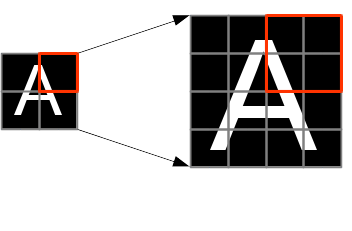
\includegraphics[scale=1]{PrintMapping.png}
\flushleft

\newpage
\begin{lstlisting}[style=c,title = Character expansion algorithm]
	void init_char_image(const char* charMap, uint32_t size, uint32_t* drawnChar)
	{
		for(uint32_t i=0; i<CHAR_BITS*size; i++)
		{
			uint32_t line = charMap[i/size];  
			// iterate through every column in teh final char image
			for(uint32_t j=0; j<CHAR_BITS*size; j++)
			{
				drawnChar[i*CHAR_BITS*size+j] = (BIT(line, 0))*WHITE_32; // BIT(val,bit) is a bit mask
				if(j%size == 0 && j>0)
					// Every size iterations we must shift the current line to select the next bit
					line = line >> 1;
			}
		}
	}
\end{lstlisting}

\begin{lstlisting}[style=C, title=Image Positioning algorithm]
	void drawChar(uint32_t *characterImage, uint32_t size, 
	uint32_t x_offset, uint32_t y_offset)
	{
		uint32_t scaling = CHAR_BITS*size;
		// transform the given coordinates from text coordinates to screen/fb coordinates
		x_offset *= scaling;
		y_offset *= scaling;
		
		// iterate through every pixel in the buffer
		for(uint32_t i=0; i<scaling; i++)
		{
			for(uint32_t j=0; j<scaling; j++)
			{
				// The current framebuffer word (a pixel)
				*(volatile uint32_t *)((main_monitor.fb_ptr & ~BUS_MASK) 
				+ ((i+y_offset)*main_monitor.virtual_width + (j+x_offset)) //map the char buffer value  
				*main_monitor.color_depth/CHAR_BITS) =   //to the fb coordinates
				// The char buffer value
				characterImage[i*scaling+j];
			}
		}
	}
\end{lstlisting}

The fully implemented print function and it's overwritten versions are defined in the \href{https://github.com/Makogan/PiOS/blob/master/source/Core/Libraries/string.c}{\notengl{string.c}} file in the PiOS.

\section{Memory allocation}

For anyone familiar with the Linux operating system, the \compl{malloc()} function should ring a bell. We took inspiration from the Linux specifications and the \compl{malloc()} function to write our own, simplistic memory allocation routine.
\\~\\
The first challenge is that the Video Core and the ARM processor share the same RAM memory, in addition to this there are multiple memory mapped peripherals, so trying to select a heap area is problematic, as one may accidentally end up writing to a protected section of memory. The memory mapped peripherals and framebuffer RAM, seem to start in high memory after \compl{0x3F000000}, an our kernel lives in low memory at around \compl{0x8000} the Salomonic solution is to take the space in between the kernel and this address as our heap space and sacrifice all other, potentially useable RAM for the sake of security.
\\~\\
After doing this we need a way to mark which sections of the memory are used and which are protected and then we need a way to allocate this memory safely. Routines compiled by C look for memory backwards (they subtract from the base address), which means that whatever reference it returns must be above a section of memory large enough to contain the data. Moreover we need an efficient way to find free memory sections in the heap. We implemented the most naive and simplistic algorithm that solves all of this problems. However the algorithm is a first fit solution, and due to it's nature it not only creates a lot of memory fragmentation, but it is also susceptible of breaking after a large, undefined number of calls. So it should eb taken as an example more than a serious solution.
\\~\\
Starting at the final address (\compl{0x3F000000}) we start creating blocks from high memory into low memory whenever memory is requested. A memory block consists of 2 parts, a memory section, corresponding to the allocated memory, and a meta data section containing the size of the block, a marker that indicates the state of the block (e.g free or locked) and a pointer to the next memory block's metadata. So allocating memory is done by iterating through all blocks, trying to find one that is free and large enough to hold the requested memory, if one is found we simply return the address immediately below the metadata, which is the first address in the memory section. If no such block is found, we see if there is enough memory from the last block to the end of the kernel space to hold the requested memory block and it's metadata, if enough memory is available we increase the heap space and create a new block, then we return the address to the memory section.
\\~\\
It is obvious from this explanation why we experience memory fragmentation and why we will eventually be unable to find appropriate blocks despite the availability of free ram. But it is a correct and working example, good enough for illustration purposes.
\\~\\
The memory allocation implementation and related subroutine is found in the \href{https://github.com/Makogan/PiOS/blob/master/source/Hardware/Memory/memory_management.cpp}{\notengl{memory\_management.cpp}} file.


\centering
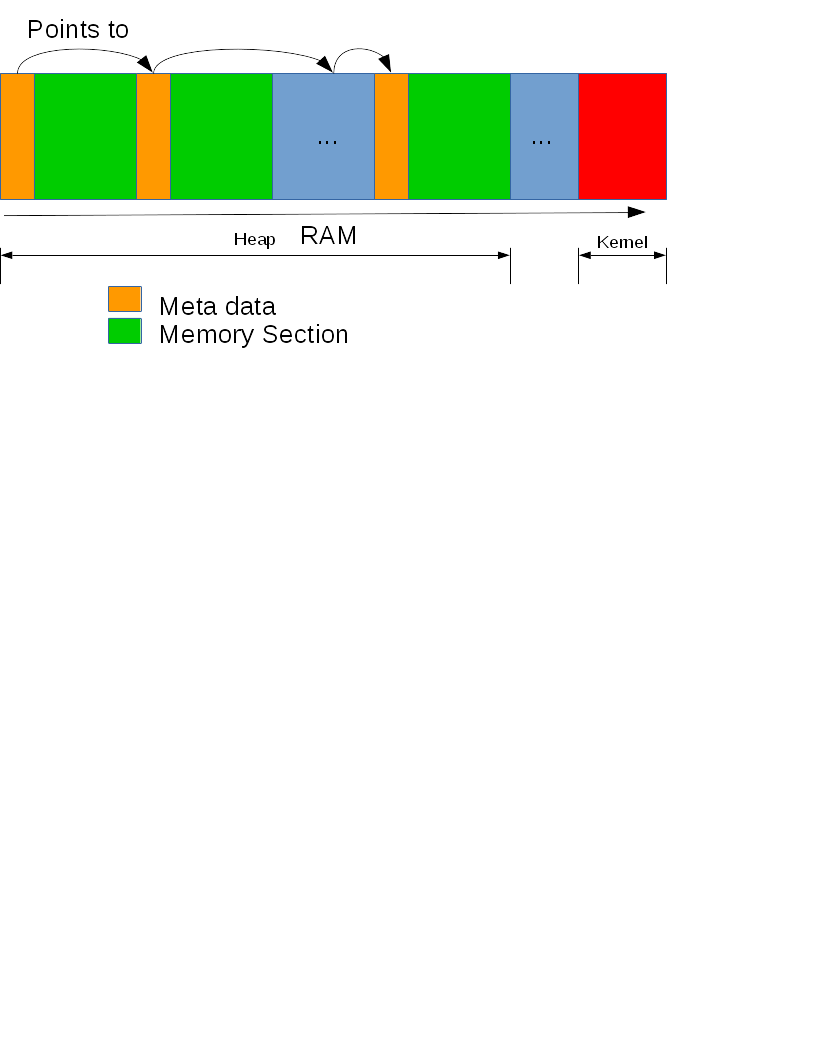
\includegraphics[scale=1]{MemoryAllocation.png}
\flushleft
\part{Epilogue, Personal reflection}

\chapter*{What I learnt}
\addcontentsline{toc}{chapter}{What I learnt}

This project certainly taught me a lot. First it forced me to learn a lot about the compilation process, before I had very little experience with make file scripts and I think I am very competent with them now, I also learnt a lot about the compilation process, the difference between executables and object files, the different compilation stages...
\\
I also learnt a lot about the \notengl{C} language it's power and it's limitations, and I think I now understand exactly why it is always said that \notengl{C} is a language for writing operating systems. It is certainly incredibly versatile, and it's one to one correspondence with assembly language makes it very suitable at imagining how the source code will be compiled and executed by the machine. 
\\~\\
I became more proficient with pointers, I was somewhat competent before, but I now understand like the back of my hand, pointer arithmetic, void pointers, the difference between pointers and references, passing by value vs passing by reference and the differences between structs and functions. For example, a mistake I did was assuming that all pointers are treated the same by \notengl{C}, and then I discovered that void pointer arithmetic is forbidden by the \notengl{C} standard, because of how pointer arithmetic works (i.e \compl{pointer\_type++} adds to the address stored in the pointer a value equal to the size of the structure or primitive it points at, so a pointer to a byte is incremented by 1 but a pointer to an integer is incremented by 4). This also makes arrays make a lot more sense now, as all that they are is a base address and a lot of pointer arithmetic.
\\~\\
Off course I also learnt a lot about low level programming, embedded systems and the ARM architecture. I know see how much I have yet to understand about low level programming but I am definitely a step ahead on that process. I could go extend this document further by enumerating all of what I learnt, but I hope that all the explanations through the document reflect it well enough, and this project report is already larger than I expected so we shall end our PiOS adventure here... Until the next time.

\chapter*{Where to go from here}
\addcontentsline{toc}{chapter}{Where to go from here}

We have just scratched the surface, and there is much more to be done. Among the things that were planned there is, creating a file system, making the kernel be able to call other programs and schedule them, implement USB drivers for basic I/O through a mouse and a keyboard, making the system dynamic by figuring the monitor dimensions dynamically instead of hard coding them for a specific resolution. Implement multi-threading and initializing the other 3 cores, creating a shell, improving the existent code, specially the memory allocation... Alas time is short and one person can only do so much. 
\\~\\
This document and code will hopefully help, however tries something like this in the future, to advance more quickly and avoid many headaches. Maybe one day the PiOS will be fully operational, but as of now, it and I both rest...

\part{Additional information}

\chapter*{Appendices}
\addcontentsline{toc}{chapter}{Appendices}
\renewcommand{\thesection}{\Alph{section}}
\setcounter{section}{0}
\section{Arm Execution Modes}
\hypertarget{arm modes}{}

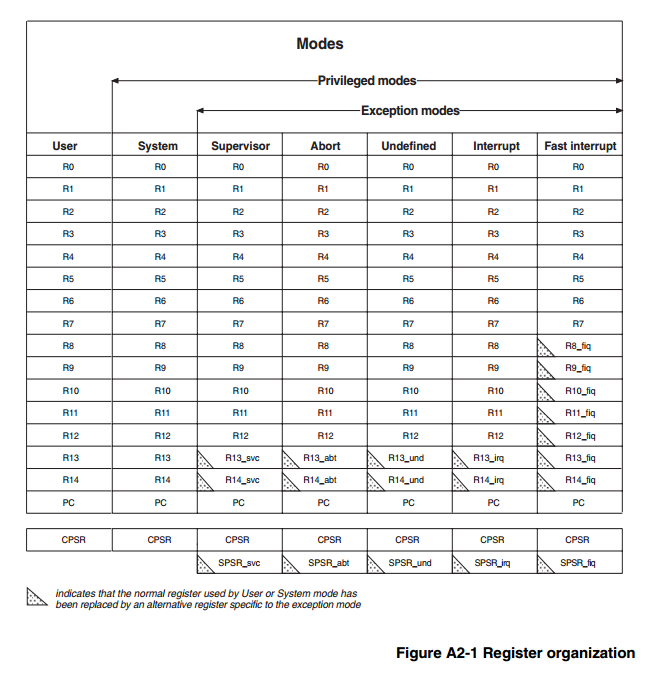
\includegraphics[scale=0.74]{ARMexecutionmodes.png}

\section{Interrupt Controller Register Map}
\hypertarget{IRQ map}{}
\begin{centering}
	\arrayrulecolor{deepblue}
	{\rowcolors{1}{lightblue!100}{pastelblue!100}
		\begin{longtable}{|l | r |}
			\hline
			 Interrupt source	&  bit number\\
			 \hline
			 \multicolumn{2}{|c|}{IRQ pending 1}\\
			 \hline
			 INTERRUPT\_TIMER0               &  0\\
			 INTERRUPT\_TIMER1               &  1\\
			 INTERRUPT\_TIMER2               &  2\\
			 INTERRUPT\_TIMER3               &  3\\
			 INTERRUPT\_CODEC0               &  4\\
			 INTERRUPT\_CODEC1               &  5\\
			 INTERRUPT\_CODEC2               &  6\\
			 INTERRUPT\_VC\_JPEG              &  7\\
			 INTERRUPT\_ISP                  &  8\\
			 INTERRUPT\_VC\_USB               &  9\\
			 INTERRUPT\_VC\_3D                &  10\\
			 INTERRUPT\_TRANSPOSER           &  11\\
			 INTERRUPT\_MULTICORESYNC0       &  12\\
			 INTERRUPT\_MULTICORESYNC1       &  13\\
			 INTERRUPT\_MULTICORESYNC2       &  14\\
			 INTERRUPT\_MULTICORESYNC3       &  15\\
			 INTERRUPT\_DMA0                 &  16\\
			 INTERRUPT\_DMA1                 &  17\\
			 INTERRUPT\_VC\_DMA2              &  18\\
			 INTERRUPT\_VC\_DMA3              &  19\\
			 INTERRUPT\_DMA4                 &  20\\
			 INTERRUPT\_DMA5                 &  21\\
			 INTERRUPT\_DMA6                 &  22\\
			 INTERRUPT\_DMA7                 &  23\\
			 INTERRUPT\_DMA8                 &  24\\
			 INTERRUPT\_DMA9                 &  25\\
			 INTERRUPT\_DMA10                &  26\\
			 INTERRUPT\_DMA11                &  27\\
			 INTERRUPT\_DMA12                &  28\\
			 INTERRUPT\_AUX                &  29\\
			 INTERRUPT\_ARM                  &  30\\
			 INTERRUPT\_VPUDMA               &  31\\
			 \hline
			\multicolumn{2}{|c|}{IRQ pending 2}\\
			\hline
			 INTERRUPT\_HOSTPORT             &  0\\
			 INTERRUPT\_VIDEOSCALER          &  1\\
			 INTERRUPT\_CCP2TX               &  2\\
			 INTERRUPT\_SDC                  &  3\\
			 INTERRUPT\_DSI0                 &  4\\
			 INTERRUPT\_AVE                  &  5\\
			 INTERRUPT\_CAM0                 &  6\\
			 INTERRUPT\_CAM1                 &  7\\
			 INTERRUPT\_HDMI0                &  8\\
			 INTERRUPT\_HDMI1                &  9\\
			 INTERRUPT\_PIXELVALVE1          &  10\\
			 INTERRUPT\_I2CSPISLV            &  11\\
			 INTERRUPT\_DSI1                 &  12\\
			 INTERRUPT\_PWA0                 &  13\\
			 INTERRUPT\_PWA1                 &  14\\
			 INTERRUPT\_CPR                  &  15\\
			 INTERRUPT\_SMI                  &  16\\
			 INTERRUPT\_GPIO0                &  17\\
			 INTERRUPT\_GPIO1                &  18\\
			 INTERRUPT\_GPIO2                &  19\\
			 INTERRUPT\_GPIO3                &  20\\
			 INTERRUPT\_VC\_I2C               &  21\\
			 INTERRUPT\_VC\_SPI               &  22\\
			 INTERRUPT\_VC\_I2SPCM            &  23\\
			 INTERRUPT\_VC\_SDIO              &  24\\
			 INTERRUPT\_VC\_UART              &  25\\
			 INTERRUPT\_SLIMBUS              &  26\\
			 INTERRUPT\_VEC                  &  27\\
			 INTERRUPT\_CPG                  &  28\\
			 INTERRUPT\_RNG                  &  29\\
			 INTERRUPT\_VC\_ARASANSDIO        &  30\\
			 INTERRUPT\_AVSPMON              &  31\\
			 \hline
			\multicolumn{2}{|c|}{IRQ pending basic}\\
			\hline
			 INTERRUPT\_ARM\_TIMER            &  0\\
			 INTERRUPT\_ARM\_MAILBOX          &  1\\
			 INTERRUPT\_ARM\_DOORBELL\_0       &  2\\
			 INTERRUPT\_ARM\_DOORBELL\_1       &  3\\
			 INTERRUPT\_VPU0\_HALTED          &  4\\
			 INTERRUPT\_VPU1\_HALTED          &  5\\
			 INTERRUPT\_ILLEGAL\_TYPE0        &  6\\
			 INTERRUPT\_ILLEGAL\_TYPE1        &  7\\
			 INTERRUPT\_PENDING1             &  8\\
			 INTERRUPT\_PENDING2             &  9\\
			 INTERRUPT\_JPEG                 &  10\\
			 INTERRUPT\_USB                  &  11\\
			 INTERRUPT\_3D                   &  12\\
			 INTERRUPT\_DMA2                 &  13\\
			 INTERRUPT\_DMA3                 &  14\\
			 INTERRUPT\_I2C                  &  15\\
			 INTERRUPT\_SPI                  &  16\\
			 INTERRUPT\_I2SPCM               &  17\\
			 INTERRUPT\_SDIO                 &  18\\
			 INTERRUPT\_UART                 &  19\\
			 INTERRUPT\_ARASANSDIO           &  20\\
			\hline
		\end{longtable}
	}
\end{centering}



\newpage
\section{Mailbox Tags}
\hypertarget{Mailbox Tags}{}
\begin{centering}
	\arrayrulecolor{deepblue}
	{\rowcolors{1}{lightblue!100}{pastelblue!100}
	\begin{longtable}{|l | r |}
		\hline
		 END &                                    0\\
		 GET\_FIRMWARE\_REVISION &                  0x00000001\\
		 
		 SET\_CURSOR\_INFO &                        0x00008010\\
		 SET\_CURSOR\_STATE &                       0x00008011\\
		 
		 GET\_BOARD\_MODEL &                        0x00010001\\
		 GET\_BOARD\_REVISION &                     0x00010002\\
		 GET\_BOARD\_MAC\_ADDRESS &                  0x00010003\\
		 GET\_BOARD\_SERIAL &                       0x00010004\\
		 GET\_ARM\_MEMORY &                         0x00010005\\
		 GET\_VC\_MEMORY &                          0x00010006\\
		 GET\_CLOCKS &                             0x00010007\\
		 GET\_POWER\_STATE &                        0x00020001\\
		 GET\_TIMING &                             0x00020002\\
		 SET\_POWER\_STATE &                        0x00028001\\
		 GET\_CLOCK\_STATE &                        0x00030001\\
		 GET\_CLOCK\_RATE &                         0x00030002\\
		 GET\_VOLTAGE &                            0x00030003\\
		 GET\_MAX\_CLOCK\_RATE &                     0x00030004\\
		 GET\_MAX\_VOLTAGE &                        0x00030005\\
		 GET\_TEMPERATURE &                        0x00030006\\
		 GET\_MIN\_CLOCK\_RATE &                     0x00030007\\
		 GET\_MIN\_VOLTAGE &                        0x00030008\\
		 GET\_TURBO &                              0x00030009\\
		 GET\_MAX\_TEMPERATURE &                    0x0003000a\\
		 GET\_STC &                                0x0003000b\\
		 ALLOCATE\_MEMORY &                        0x0003000c\\
		 LOCK\_MEMORY &                            0x0003000d\\
		 UNLOCK\_MEMORY &                          0x0003000e\\
		 RELEASE\_MEMORY &                         0x0003000f\\
		 EXECUTE\_CODE &                           0x00030010\\
		 EXECUTE\_QPU &                            0x00030011\\
		 SET\_ENABLE\_QPU &                         0x00030012\\
		 GET\_DISPMANX\_RESOURCE\_MEM\_HANDLE &       0x00030014\\
		 GET\_EDID\_BLOCK &                         0x00030020\\
		 GET\_CUSTOMER\_OTP &                       0x00030021\\
		 GET\_DOMAIN\_STATE &                       0x00030030\\
		 SET\_CLOCK\_STATE &                        0x00038001\\
		 SET\_CLOCK\_RATE &                         0x00038002\\
		 SET\_VOLTAGE &                            0x00038003\\
		 SET\_TURBO &                              0x00038009\\
		 SET\_CUSTOMER\_OTP &                       0x00038021\\
		 SET\_DOMAIN\_STATE &                       0x00038030\\
		 GET\_GPIO\_STATE &                         0x00030041\\
		 SET\_GPIO\_STATE &                         0x00038041\\
		 SET\_SDHOST\_CLOCK &                       0x00038042\\
		 GET\_GPIO\_CONFIG &                        0x00030043\\
		 SET\_GPIO\_CONFIG &                        0x00038043\\

		 ALLOCATE &                   0x00040001\\
		 BLANK\_SCREEN &               0x00040002\\
		 GET\_PHYSICAL\_WIDTH\_HEIGHT &  0x00040003\\
		 GET\_VIRTUAL\_WIDTH\_HEIGHT &   0x00040004\\
		 GET\_DEPTH &                  0x00040005\\
		 GET\_PIXEL\_ORDER &            0x00040006\\
		 GET\_ALPHA\_MODE &             0x00040007\\
		 GET\_PITCH &                  0x00040008\\
		 GET\_VIRTUAL\_OFFSET &         0x00040009\\
		 GET\_OVERSCAN &               0x0004000a\\
		 GET\_PALETTE &                0x0004000b\\
		 GET\_TOUCHBUF &               0x0004000f\\
		 GET\_GPIOVIRTBUF &            0x00040010\\
		 RELEASE &                    0x00048001\\
		 TEST\_PHYSICAL\_WIDTH\_HEIGHT & 0x00044003\\
		 TEST\_VIRTUAL\_WIDTH\_HEIGHT &  0x00044004\\
		 TEST\_DEPTH &                 0x00044005\\
		 TEST\_PIXEL\_ORDER &           0x00044006\\
		 TEST\_ALPHA\_MODE &            0x00044007\\
		 TEST\_VIRTUAL\_OFFSET &        0x00044009\\
		 TEST\_OVERSCAN &              0x0004400a\\
		 TEST\_PALETTE &               0x0004400b\\
		 TEST\_VSYNC &                 0x0004400e\\
		 SET\_PHYSICAL\_WIDTH\_HEIGHT &  0x00048003\\
		 SET\_VIRTUAL\_WIDTH\_HEIGHT &   0x00048004\\
		 SET\_DEPTH &                  0x00048005\\
		 SET\_PIXEL\_ORDER &            0x00048006\\
		 SET\_ALPHA\_MODE &             0x00048007\\
		 SET\_VIRTUAL\_OFFSET &         0x00048009\\
		 SET\_OVERSCAN &               0x0004800a\\
		 SET\_PALETTE &                0x0004800b\\
		 SET\_TOUCHBUF &               0x0004801f\\
		 SET\_GPIOVIRTBUF &            0x00048020\\
		 SET\_VSYNC &                  0x0004800e\\
		 SET\_BACKLIGHT &              0x0004800f\\
		 
		 VCHIQ\_INIT &                 0x00048010\\
		 
		 GET\_COMMAND\_LINE &           0x00050001\\
		 GET\_DMA\_CHANNELS &           0x00060001\\
		 \hline
	\end{longtable}
}
\end{centering}

\begin{thebibliography}{9}
	\addcontentsline{toc}{chapter*}{References}
	
	\bibitem{Leon de Boer}
	\href{https://www.raspberrypi.org/forums/memberlist.php?mode=viewprofile&u=213434}{Leon de Boer}, through multiple posts in the Raspberry Pi forums. 
	
	
	\bibitem{Valvers} 
		Brian Sidebotham 
	\textit{\href{http://www.valvers.com/open-software/raspberry-pi/step01-bare-metal-programming-in-cpt1/}{Valvers Raspberry Pi tutorial}}.
	\\\texttt{http://www.valvers.com/open-software/raspberry-pi/step01-bare
		-metal-programming-in-cpt1/}
	
	\bibitem{359} 
	Jalal Kawash,
	\textit{Computer Machinery 2 [CPSC 359]} winter 2016, University of Calgary.
	
	\bibitem{ARM info}
	The ARM \href{http://infocenter.arm.com/help/index.jsp}{info center}
	\\\texttt{http://infocenter.arm.com/help/index.jsp}
	
	\bibitem{xinu}
	Embedded Xinu \href{http://embedded-xinu.readthedocs.io/en/latest/arm/rpi/}{documentation}
	\\\texttt{http://embedded-xinu.readthedocs.io/en/latest/arm/rpi/}
	
	\bibitem{linux}
	Raspberry Pi Linux kernel \href{https://github.com/raspberrypi/linux/tree/rpi-3.6.y/arch/arm/mach-bcm2708}{source code}
	\\\texttt{https://github.com/raspberrypi/linux/tree/rpi-3.6.y/arch/arm/mach-bcm2708}
	\bibitem{Mailbox}
	
	The official Raspberry Pi \href{https://github.com/raspberrypi/firmware/wiki/Mailbox-property-interface}{Github Repository}
	\\\texttt{https://github.com/raspberrypi/firmware/wiki/Mailbox-property-interface}
	
	\bibitem{Marwan Burelle}
	Marwan Burelle, \textit{\href{http://www.inf.udec.cl/~leo/Malloc_tutorial.pdf}{A malloc tutorial}}, February 16, 2009
	
	\bibitem{linaro}
	Ken Werner, \textit{\href{https://wiki.linaro.org/KenWerner/Sandbox/libunwind?action=AttachFile&do=get&target=libunwind-LDS.pdf}{Stack Frame Unwinding on ARM}}, Budapest 2011 \\\texttt{https://wiki.linaro.org/KenWerner/Sandbox/libunwind?action=
		AttachFile\&do=get\&target=libunwind-LDS.pdf}
	
	\bibitem{forumns}
	Raspberry Pi \href{https://www.raspberrypi.org/forums/}{forums}
	\\\texttt{https://www.raspberrypi.org/forums/}
\end{thebibliography}

\newpage
\vspace*{\fill}
\centering
\Huge|\textit{``Live long and propser"}, 
\\~\\
\Large Spock
\vspace*{\fill}
\end{document}
